%\addcontentsline{toc}{chapter}{Flight Dynamics}
\chapter{Flight dynamics}
\label{ch:FlightDynamics}

\section{Overview}
In order to design a receiver able to cope with high dynamics experienced during space flight, it is crucial to have an understanding of the types of dynamics the receiver is likely to encounter. Based on a thorough analysis of a range of Launch Services User's Guide published by commercial space flight operators, the following phases of flight have been identified as exhibiting the most severe dynamics: 

\begin{enumerate}
\item{Launch}
\item{Stage separation}
\item{Re-entry}
\end{enumerate}

\subsection{Launch}
Launch is the most obvious case of dynamics that a \ac{GNSS} receiver would experience. Axial accelerations of 6 g are experienced with most launch vehicles, up to 13 g in the case of the Minotaur rocket. During ascent, accelerations of 2 g due to crosswinds and course corrections may be experienced. An overview of the launch dynamics experience by a range of acceleration that a \ac{SV} will experience can be found in table \ref{QSLTable}.

\begin{figure}[!htb] 
    \centering
    \includegraphics[width=1\textwidth]{FlightDynamics/SoyuzAcceleration.png} 
    \caption{Typical longitudinal acceleration experienced by the Soyuz payload. Note the significant change in acceleration (jerk) upon stage separation. Image from \cite{Soyuz}.}
    \label{fig:SoyuzAcceleration}
\end{figure}

\begin{figure}[!htb] 
    \centering
    \includegraphics[width=1\textwidth]{FlightDynamics/SoyuzRelativeVelocity.png} 
    \caption{Typical Soyuz velocity profile. Noticed that 3 separate stages, and 2 stage separation events can be observed in this plot. Image from \cite{Soyuz}.}
    \label{fig:SoyuzRelativeVelocity}
\end{figure}



\begin{table}[!htb]
\centering
\begin{tabular}{|l|l|l|}
\hline
\rowcolor[HTML]{C0C0C0} 
Space Vehicle       & Axial                   & Lateral                \\ \hline
Ariane 5            & 4.6 g \cite{Ariane}     & 2.0 g \cite{Ariane}    \\ \hline
\rowcolor[HTML]{EFEFEF} 
Atlas V 400         & 5.0 g \cite{AtlasV}     & 2.0 g \cite{AtlasV}    \\ \hline
Atlas V 500         & 4.6 g \cite{AtlasV}     & 2.0 g \cite{AtlasV}    \\ \hline
\rowcolor[HTML]{EFEFEF} 
Delta IV Medium     & 6.0 g \cite{DeltaIV}    & 2.0 g \cite{DeltaIV}   \\ \hline
Delta IV Heavy      & 5.5 g \cite{DeltaIV}    & 2.0 g \cite{DeltaIV}   \\ \hline
\rowcolor[HTML]{EFEFEF} 
Falcon 9 Revision 0 & 6.0 g \cite{Falcon9}    & 2.0 g \cite{Falcon9}   \\ \hline
Minotaur            & 13.0 g  \cite{Minotaur} & 12.0 g \cite{Minotaur} \\ \hline
\rowcolor[HTML]{EFEFEF} 
Soyuz               & 5.0 g \cite{Soyuz}      & 1.8 g \cite{Soyuz}     \\ \hline
\end{tabular}
\caption{Maximum \ac{QSL} experienced during launch.}
\label{QSLTable}
\end{table}



\subsection{Stage separation}

Significant shocks can be generated during stage separation, due to pyrotechnic events and fairing jettison\cite{AtlasV,Ariane,DeltaIV}. While these shocks have no impact on the line of sight dynamics experienced by the receiver, they do have an impact on the crystal. Mechanical vibrations can modulate the output frequency of the crystal, placing stress on the tracking loops. A mission profile for a Minotaur rocket can be seen in figure \ref{fig:MinotaurMissionProfile}.


\begin{figure}[!htb] 
    \centering
    \includegraphics[width=1\textwidth]{FlightDynamics/MinotaurMissionProfile.png} 
    \caption{A typically Minotaur mission profile, note there are 5 unique separation events. Image from \cite{Minotaur}}
    \label{fig:MinotaurMissionProfile}
\end{figure}

\subsection{Re-entry}
Getting to space is only half the challenge. Accurate guidance during re-entry is crucial to reducing costs in the space industry. Most \ac{SV}'s are currently employed to launch satellites, however manned missions regularly return capsules to earth. The maximum design acceleration experienced can be seen in table \ref{ReEntryTable}. 

During re-entry, the extreme temperatures ionises the gasses surrounding the vehicle, forming  layer of plasma. This layer of plasma severely attenuates radio signals, resulting in what is termed 'reentry blackout'. GNSS receiver design presents an inherent trade off between sensitivity and high dynamics performance. It is likely that the receiver will loose track of the the signal, and be forced to re-acquire at a lower altitude, once the plasma has subsided. 

\begin{table}[!htb]
\centering
\begin{tabular}{|l|l|}
\hline
\rowcolor[HTML]{C0C0C0} 
Space Vehicle & Peak acceleration                    \\ \hline
Gemini        & 12 g \cite{FAA}                      \\ \hline
\rowcolor[HTML]{EFEFEF} 
Apollo        & 7.19 g \cite{johnston1975biomedical} \\ \hline
Dragon        & 5.0 g \cite{trevino2008spacex}       \\ \hline
\rowcolor[HTML]{EFEFEF} 
Soyuz         & 10 g \cite{ReentryDynamics}          \\ \hline
\end{tabular}
\caption{Peak acceleration experienced by different \ac{SV}'s during re-entry}. It is useful to correlate this information with figure \ref{fig:MaxReentryAcceleration}.
\label{ReEntryTable}
\end{table}


The maximum acceleration experienced during re-entry can be closely approximated parametrically using the following equation from \cite{eastre}: 

\begin{equation}
(\frac{dv}{dt})_{max} = \frac{\beta V_0^2}{2e} \sin \gamma_0
\end{equation}

Where:
\begin{align*}
V_0 &= \text{Velocity prior to entering atmosphere}\\
 \beta &= \text{Atmospheric scale height}\\
       &= 0.000139 m^{-1}\\
\gamma &= \text{Vehicle's flight-path angle (deg or rad)}\\
     e &= \text{Base of the natural logarithm}\\
       &= 2.7182\ldots
\end{align*}

This convenient formula provides an intuitive understanding of how the maximum acceleration varies with velocity, as well as allowing performance to be estimated, when official figures are not published. A contour plot which can be used for reference can be found in figure \ref{fig:MaxReentryAcceleration}.


\begin{figure}[!htb] 
    \centering
    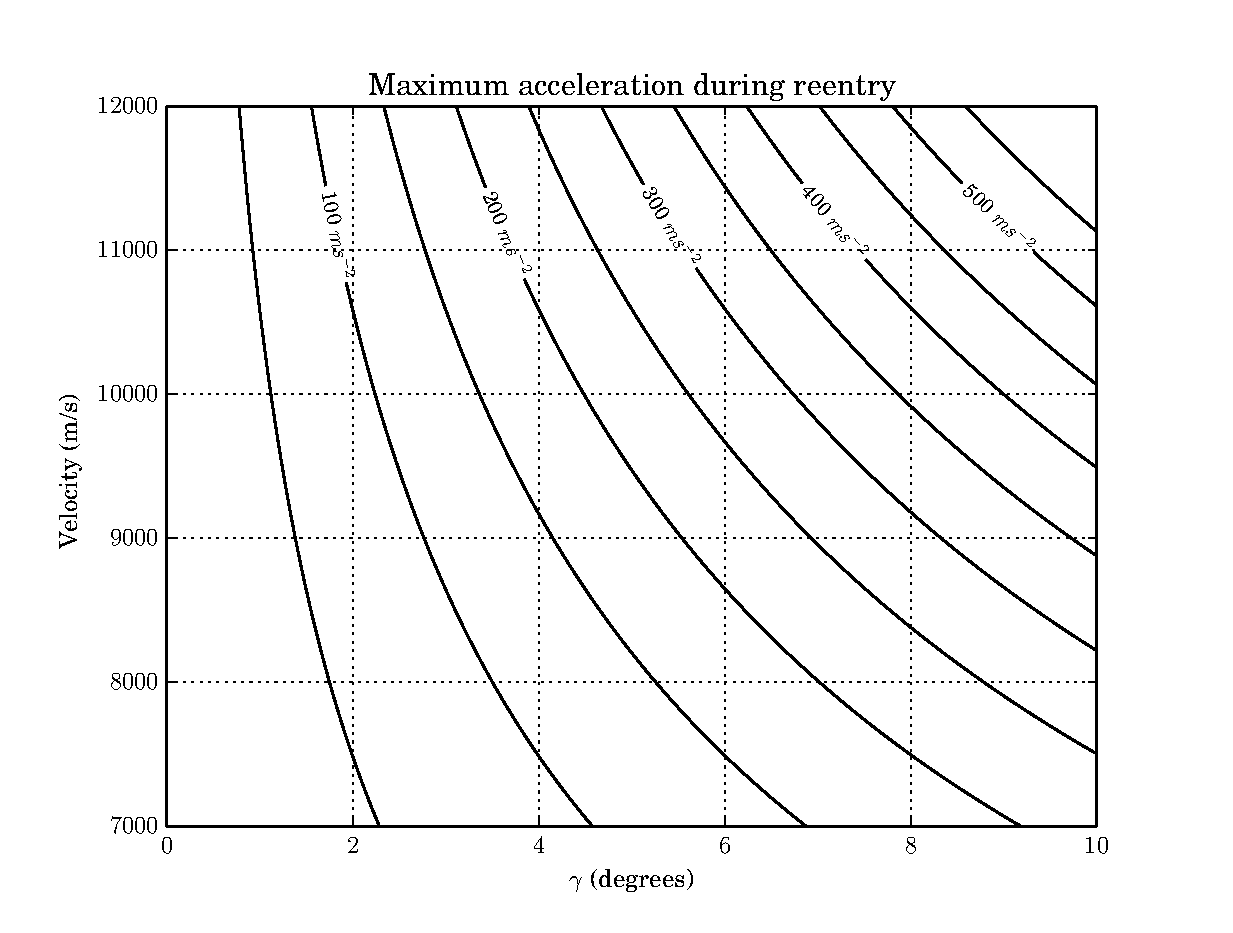
\includegraphics[width=1\textwidth]{FlightDynamics/MaxAcceleration.eps} 
    \caption{A contour plot of the maximum acceleration experienced during reentry.}
    \label{fig:MaxReentryAcceleration}
\end{figure}


